% ==============================================================================
% 第二章: 卡诺图 - 找茬游戏
% ==============================================================================
\section{卡诺图 (找茬游戏)}

\begin{hack}[K-Map就是找茬游戏!]
\textbf{三步走:}
\begin{enumerate}
\item \textbf{填图}:看到变量就填1
\item \textbf{圈图}:把1圈起来(越大越好)
\item \textbf{写式}:圈里不变的变量写出来
\end{enumerate}
\end{hack}

\subsection{4变量K-Map模板 (照着画!)}

\begin{center}
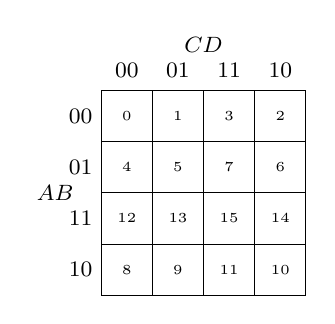
\begin{tikzpicture}[scale=0.65]
\draw (0,0) grid (4,4);
% 列标签 CD
\node at (0.5, 4.4) {\footnotesize 00};
\node at (1.5, 4.4) {\footnotesize 01};
\node at (2.5, 4.4) {\footnotesize 11};
\node at (3.5, 4.4) {\footnotesize 10};
\node at (2, 4.9) {\footnotesize $CD$};
% 行标签 AB
\node at (-0.4, 3.5) {\footnotesize 00};
\node at (-0.4, 2.5) {\footnotesize 01};
\node at (-0.4, 1.5) {\footnotesize 11};
\node at (-0.4, 0.5) {\footnotesize 10};
\node at (-0.9, 2) {\footnotesize $AB$};
% 索引号
\node at (0.5,3.5) {\tiny 0};
\node at (1.5,3.5) {\tiny 1};
\node at (2.5,3.5) {\tiny 3};
\node at (3.5,3.5) {\tiny 2};
\node at (0.5,2.5) {\tiny 4};
\node at (1.5,2.5) {\tiny 5};
\node at (2.5,2.5) {\tiny 7};
\node at (3.5,2.5) {\tiny 6};
\node at (0.5,1.5) {\tiny 12};
\node at (1.5,1.5) {\tiny 13};
\node at (2.5,1.5) {\tiny 15};
\node at (3.5,1.5) {\tiny 14};
\node at (0.5,0.5) {\tiny 8};
\node at (1.5,0.5) {\tiny 9};
\node at (2.5,0.5) {\tiny 11};
\node at (3.5,0.5) {\tiny 10};
\end{tikzpicture}
\end{center}

\textbf{格雷码顺序:00, 01, 11, 10} (背下来!)

\subsection{填图口诀}

\begin{hack}[看到变量往哪填?]
\textbf{4变量ABCD的位置:}
\begin{itemize}
\item $A=1$:下两行 (row 11, 10)
\item $B=1$:中间两行 (row 01, 11)
\item $C=1$:中间两列 (col 01, 11)
\item $D=1$:右边两列 (col 11, 10)
\end{itemize}

\textbf{Not变量:} $\bar{A}$就是$A=0$的区域,取反!
\end{hack}

\subsection{圈图无脑法}

\begin{hack}[四种必会的圈法]
\textbf{1. 四角圈} = $\bar{B}\bar{D}$
\begin{center}
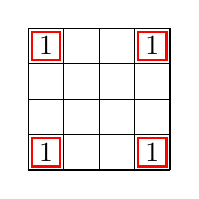
\begin{tikzpicture}[scale=0.45]
\draw (0,0) grid (4,4);
\node at (0.5,3.5) {1}; \node at (3.5,3.5) {1};
\node at (0.5,0.5) {1}; \node at (3.5,0.5) {1};
\draw[red,thick] (0.1,3.1) rectangle (0.9,3.9);
\draw[red,thick] (3.1,3.1) rectangle (3.9,3.9);
\draw[red,thick] (0.1,0.1) rectangle (0.9,0.9);
\draw[red,thick] (3.1,0.1) rectangle (3.9,0.9);
\end{tikzpicture}
\end{center}

\textbf{2. 一整行} = 只有AB变
\begin{center}
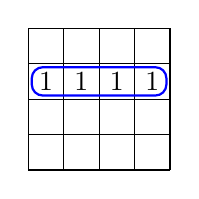
\begin{tikzpicture}[scale=0.45]
\draw (0,0) grid (4,4);
\node at (0.5,2.5) {1}; \node at (1.5,2.5) {1};
\node at (2.5,2.5) {1}; \node at (3.5,2.5) {1};
\draw[blue,thick,rounded corners] (0.1,2.1) rectangle (3.9,2.9);
\end{tikzpicture}
\end{center}

\textbf{3. 田字格(4个)} = 消两个变量

\textbf{4. 上下卷/左右卷} = 可以跨边界!
\end{hack}

\subsection{圈图规则}

\begin{pitfall}[圈图三铁律]
\begin{enumerate}
\item 圈的大小必须是 \textbf{2的幂}:1,2,4,8,16
\item 圈\textbf{越大越好}(消去更多变量)
\item 每个1\textbf{至少被圈一次}
\end{enumerate}
\end{pitfall}

\subsection{从圈写表达式}

\begin{hack}[圈里不变的写出来!]
\textbf{看圈内的变量值:}
\begin{itemize}
\item 变量全是1 $\to$ 写变量本身
\item 变量全是0 $\to$ 写变量的NOT
\item 变量有0有1 $\to$ 不写(被消掉了)
\end{itemize}

\textbf{例:} 圈在AB=01, CD=任意
\begin{itemize}
\item A全是0 $\to$ 写$\bar{A}$
\item B全是1 $\to$ 写$B$
\item CD有0有1 $\to$ 不写
\item \textbf{结果:$\bar{A}B$}
\end{itemize}
\end{hack}

\subsection{异或的秘密}

\begin{hack}[看到棋盘格 = XOR!]
如果K-Map里1和0像国际象棋棋盘一样交错:

\begin{center}
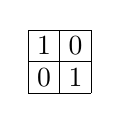
\begin{tikzpicture}[scale=0.4]
\draw (0,0) grid (2,2);
\node at (0.5,1.5) {1}; \node at (1.5,1.5) {0};
\node at (0.5,0.5) {0}; \node at (1.5,0.5) {1};
\end{tikzpicture}
\end{center}

\textbf{直接写:} $A \oplus B$ (异或)

这种情况\textbf{没法化简},别浪费时间圈了!
\end{hack}

\subsection{Don't Care}

\begin{keybox}[X可以当1也可以当0]
\begin{itemize}
\item 能让圈变大 $\to$ 当1
\item 不能 $\to$ 当0忽略
\end{itemize}
目标:让圈尽量大!
\end{keybox}
